\date{}
\title{}
\date{}
\begin{document}
\begin{frame}
    \titlepage
\end{frame}


\makeatletter
\newenvironment<>{btHighlight}[1][]
{\begin{onlyenv}#2\begingroup\tikzset{bt@Highlight@par/.style={#1}}\begin{lrbox}{\@tempboxa}}
{\end{lrbox}\bt@HL@box[bt@Highlight@par]{\@tempboxa}\endgroup\end{onlyenv}}

\newcommand<>\btHL[1][]{%
  \only#2{\begin{btHighlight}[#1]\bgroup\aftergroup\bt@HL@endenv}%
}
\def\bt@HL@endenv{%
  \end{btHighlight}%   
  \egroup %
}
\tikzset{
    btHLbox/.style={
        fill=red!30,outer sep=0pt,inner xsep=1pt, inner ysep=0pt, rounded corners=3pt
    },
}
\newcommand{\bt@HL@box}[2][]{%
  \tikz[#1]{%
    \pgfpathrectangle{\pgfpoint{1pt}{0pt}}{\pgfpoint{\wd #2}{\ht #2}}%
    \pgfusepath{use as bounding box}%
    \node[text width={},draw=none,anchor=base west, btHLbox, minimum height=\ht\strutbox+1pt,#1]{\raisebox{1pt}{\strut}\strut\usebox{#2}};
  }%
}

\lst@CCPutMacro
    \lst@ProcessOther {"2A}{%
      \lst@ttfamily 
         {\raisebox{2pt}{*}}% used with ttfamily
         {\raisebox{2pt}{*}}}% used with other fonts
    \@empty\z@\@empty

\lstdefinelanguage
   [x8664gas]{Assembler}     % add a "x64" dialect of Assembler
   [x86masm]{Assembler} % based on the "x86masm" dialect
   % with these extra keywords:
   {morekeywords={CDQE,CQO,CMPSQ,CMPXCHG16B,JRCXZ,LODSQ,MOVSXD,%
                  POPFQ,PUSHFQ,SCASQ,STOSQ,IRETQ,RDTSCP,SWAPGS,.TEXT,.STRING,.ASCIZ,%
                  BEQ,LW,SW,LB,SB,ADDIU,J,BEQZ,BNEZ,BNE,%
                  MOVUPD,MULPD,MOVSD,MULSD,%
                  SHLADD,MOV,CMP.LT,TBIT.NZ,BR.RET.SPTK.MANY,%
                  ADDQ,POPQ,PUSHQ,RRMOVQ,MRMOVQ,RMMOVQ,IRMOVQ,%
                  <-,LL,SC,ADDI,ADDL,VMOVDQA,ADDQ,CMPL,JB,JBE,MOVL,CLTQ,
                  MOVW,PUSHW,MOV,ADD,SUB,INT,PUSH,MOV,ADD,REP,MOVSB,%
                  TESTQ,CMPQ,MOVL,MOVQ,ADDQ,JMPQ,XORQ,%
                  LEAQ,LEAL,LEA,RETQ,RET,POPL,POPW,PUSHL,PUSHW,%
                  LEAW,%
                  SUBQ,SYSCALL,.ASCII,CALLQ,MOVSLQ,JMP,ANDQ,SHRQ,MOVB,INCQ,TESTL,XORL,%
                  SHRL,LEAL,SARL,SUBL,IMULL,IMULQ,MOVDQU,PADDD,XORL,%
                  MOVZBL,MOVZB,SHRB,SRAL,SHRL,ANDL,%
                  CMOVNS,SRAL,SRAQ,MOVZBW,MOVZBQ,%
                  PADDW,PADDQ,MODUPS,MOVAPD,%
                  MOVL,RET,.GLOBL,%
                  },
    deletekeywords={eax,ebx,sp,si,cx,di,ds,cs,es,fs,dx,ax,bx,al,esi,ebp,ecx,rip,eip,edx,edi,rdi,esp},
    morecomment=[l]{\#},
    morecomment=[l]{\/\/},
    morecomment=[s]{/*}{*/},
    sensitive=false,
    keepspaces=true} % et

\lstalias[]{myasm}[x8664gas]{Assembler}

\lstdefinelanguage{JavaScript}{
  keywords={typeof, new, true, false, catch, function, return, null, catch, switch, var, if, in, while, do, else, case, break},
  ndkeywords={class, export, boolean, throw, implements, import, this},
  sensitive=false,
  comment=[l]{//},
  morecomment=[s]{/*}{*/},
  morestring=[b]',
  morestring=[b]"
}

\newcommand{\keywordstyle}{\sourcecodeprolight\bfseries\color{blue!30!black}}
\newcommand{\stringstyle}{\color{blue!20!black}\ttfamily}

\lstset{
    language=C,
    basicstyle=\sourcecodepro\EmptyMapping,
    escapechar=`,
    keywordstyle=\keywordstyle\EmptyMapping,
    identifierstyle=\sourcecodepro\EmptyMapping,
    numberstyle=\small\color{black!70},
    commentstyle=\color{red!60!black}\ttfamily\itshape,
    stringstyle=\color{blue!20!black}\ttfamily,
    ndkeywordstyle=\bfseries\color{blue!30!black},
    upquote=true,
}



\lstdefinestyle{medium}{
    basicstyle=\sourcecodepro\EmptyMapping\fontsize{12}{13}\selectfont,
    keywordstyle=\sourcecodepro\EmptyMapping\fontsize{12}{13}\selectfont\keywordstyle,
}

\lstdefinestyle{small}{
    basicstyle=\sourcecodepro\EmptyMapping\small,
    keywordstyle=\sourcecodepro\EmptyMapping\small\keywordstyle,
}

\lstdefinestyle{smaller}{
    basicstyle=\sourcecodepro\EmptyMapping\fontsize{11}{12}\selectfont,
    keywordstyle=\sourcecodepro\EmptyMapping\fontsize{11}{12}\selectfont\keywordstyle,
}


\lstdefinestyle{script}{
    basicstyle=\sourcecodepro\EmptyMapping\scriptsize,
    keywordstyle=\sourcecodepro\EmptyMapping\scriptsize\bfseries,
}




\begin{frame}{last time}
    \begin{itemize}
        \item static and dynamic (AKA shared) libraries
            \begin{itemize}
            \item static = in executable
            \item shared = load when program starts
            \item \texttt{ar} to build static; \texttt{-fPIC}/\texttt{-shared} to build shared
            \end{itemize}
        \item makefile rules
            \begin{itemize}
            \item target: prereq
            \item tab-prefixed commands
            \item `chains' of rules
            \end{itemize}
    \end{itemize}
\end{frame}

\section{building, con't}

\subsection{exercise}
\begin{FragileFrame}
\frametitle{exericse setup}
    \begin{itemize}
    \item a program has source files compiler.c, main.c, functions.customlang
    \item compiler.c builds a custom compiler
    \item functions.customlang needs to be compiled with that compiler
    \item so normal build process is:
\begin{Verbatim}[frame=single,fontsize=\fontsize{12}{13}]
clang -c compiler.c
clang -c main.c
clang -o compiler compiler.o
./compiler -c functions.customlang
clang -o program main.o functions.o
\end{Verbatim}
    \end{itemize}
\end{FragileFrame}

\begin{FragileFrame}
\frametitle{exercise part 1}
\begin{Verbatim}[frame=single,fontsize=\fontsize{13}{14}]
clang -c compiler.c
clang -c main.c
clang -o compiler compiler.o
./compiler -c functions.customlang
clang -o program main.o functions.o
\end{Verbatim}
    \begin{itemize}
    \item besides \texttt{program}, \texttt{main.o}, makefile should have what targets?
\begin{tabular}{ll}
    A. \texttt{functions.customlang} & B. \texttt{functions.o} \\
    C. \texttt{compiler.o} & D. \texttt{compiler} \\
    E. all of the above & F. B and C \\
    G. A and B and D & H. B and C and D \\
    I. something else 
\end{tabular}
    \end{itemize}
\end{FragileFrame}

\begin{FragileFrame}
\frametitle{exercise part 2}
\begin{Verbatim}[frame=single,fontsize=\fontsize{12}{13}]
clang -c compiler.c
clang -c main.c
clang -o compiler compiler.o
./compiler -c functions.customlang
clang -o program main.o functions.o
\end{Verbatim}
    \begin{itemize}
    \item part 2: make rule for functions.o? first blank = ???
\begin{Verbatim}[frame=single,fontsize=\fontsize{11}{12}]
functions.o: ____________________________________
▶     _____________________________________
\end{Verbatim}
\begin{tabular}{llll}
A. & \texttt{functions.customlang} & B. & \texttt{functions.customlang compiler} \\
C. & \texttt{compiler} & D. & \texttt{functions.customlang compiler.o} \\
E. & \texttt{functions.c} & F. & \texttt{program} \\
G. & something else\\
\end{tabular}
    \end{itemize}
\end{FragileFrame}

\begin{FragileFrame}
\frametitle{exercise part 3}
\begin{Verbatim}[frame=single,fontsize=\fontsize{13}{14}]
clang -c compiler.c #1
clang -c main.c #2
clang -o compiler compiler.o #3
./compiler -c functions.customlang #4
clang -o program main.o functions.o #5
\end{Verbatim}
    \begin{itemize}
    \item command 1 goes in rule for which target? command 3? 4?
\begin{tabular}{lll}
    A. \texttt{compiler.o} & B. \texttt{main.o} & C. \texttt{compiler} \\
    D. \texttt{functions.o} & E. \texttt{program} & F. something else \\
\end{tabular}
    \end{itemize}
\end{FragileFrame}



\subsection{phony targets}

\begin{frame}{`phony' targets (1)}
\begin{itemize}
\item common to have Makefile targets that aren't files
\end{itemize}
{\tt
\begin{tabular}{l}
all: program1 program2 libfoo.a \\
\end{tabular}
}
\begin{itemize}
\item ``\texttt{make all}'' effectively shorthand for ``\texttt{make program1 program2 libfoo.a}''
\item no actual file called ``all''
\end{itemize}
\end{frame}


\begin{frame}{`phony' targets (2)}
\begin{itemize}
\item sometimes want targets that don't actually build file
\item example: ``\texttt{make clean}'' to remove generated files
\end{itemize}
{\tt
\begin{tabular}{l}
clean: \\
▶\hspace{3cm}rm --force main.o extra.o \\
\end{tabular}
}
\end{frame}

\begin{frame}{but what if I create\ldots}

{\tt
\begin{tabular}{l}
clean: \\
▶\hspace{3cm}rm --force main.o extra.o \\
~ \\
all: program1 program2 libfoo.a \\
\end{tabular}
}
\begin{itemize}
\item Q: if I make a file called ``all'' and then ``make all'' what happens?
\item Q: same with ``clean'' and ``make clean''?
\end{itemize}
\end{frame}

\begin{frame}{marking phony targets}

{\tt
\begin{tabular}{l}
clean: \\
▶\hspace{3cm}rm --force main.o extra.o \\
~ \\
all: program1 program2 libfoo.a \\
~ \\
\myemph{.PHONY: all clean}
\end{tabular}
}
\begin{itemize}
\item special .PHONY rule says `` `all' and `clean' not real files''
\vspace{.5cm}
\item \small (not required by POSIX, but in every \texttt{make} version I know)
\end{itemize}
\end{frame}



\subsection{conventional targets}

\begin{frame}{conventional targets}

common convention: \\
\begin{tabular}{l|l}
target name & purpose \\
(default), \texttt{all} & build everything \\
\texttt{install} & install to standard location \\
\texttt{test} & run tests \\
\texttt{clean} & remove generated files \\
\end{tabular}
\end{frame}


\subsection{variables, macro rules}

\begin{frame}{redundancy (1)}

{\tt
\begin{tabular}{l}
program: main.o extra.o \\
▶\hspace{1.5cm}clang -Wall -o program main.o extra.o \\
~ \\
extra.o: extra.c extra.h \\
▶\hspace{1.5cm}clang -Wall -o extra.o -c extra.c \\
main.o: main.c main.h extra.h \\
~ \\
▶\hspace{1.5cm}clang -o main.o -c main.c \\
\end{tabular}
}
\begin{itemize}
\item what if I want to run \texttt{clang} with \texttt{-fsanitize=address} instead of \texttt{-Wall}?
\item what if I want to change \texttt{clang}to \texttt{gcc}?
\end{itemize}
\end{frame}

\begin{frame}{variables/macros (1)}

{\tt\small
\begin{tabular}{l}
\myemph{CC = gcc} \\
\myemph{CFLAGS = -Wall -pedantic -std=c11 -fsanitize=address} \\
\myemph{LDFLAGS = -Wall -pedantic -fsanitize=address} \\
\myemph{LDLIBS = -lm} \\
~ \\
program: main.o extra.o \\
▶\hspace{1.5cm}\$(CC) \$(LDFLAGS) -o program main.o extra.o \$(LDLIBS) \\
~ \\
extra.o: extra.c extra.h \\
▶\hspace{1.5cm}\$(CC) \$(CFLAGS) -o extra.o -c extra.c \\
~ \\
main.o: main.c main.h extra.h \\
▶\hspace{1.5cm}\$(CC) \$(CFLAGS) -o main.o -c main.c \\
\end{tabular}
}
\end{frame}

\begin{frame}{aside: conventional names}
\begin{itemize}
\item chose names \texttt{CC}, \texttt{CFLAGS}, \texttt{LDFLAGS}, etc.
\item not required, but conventional names (incomplete list follows)
\end{itemize}
\begin{tabular}{ll}
\texttt{CC} & C compiler \\
\texttt{CFLAGS} & C compiler options \\
\texttt{LDFLAGS} & linking options \\
\texttt{LIBS} or \texttt{LDLIBS} & libraries \\
\end{tabular}
\end{frame}

\begin{frame}{variables/macros (2)}

{\small\tt
\begin{tabular}{l}
CC = gcc \\
CFLAGS = -Wall \\
LDFLAGS = -Wall \\
LDLIBS = -lm \\
~ \\
program: main.o extra.o \\
▶\hspace{1.5cm}\$(CC) \$(LDFLAGS) -o \myemph{\$@} \myemph{\$\textasciicircum} \$(LDLIBS) \\
~ \\
extra.o: extra.c extra.h \\
▶\hspace{1.5cm}\$(CC) \$(CFLAGS) -o \myemph{\$@} -c \myemph{\$<} \\
~ \\
main.o: main.c main.h extra.h \\
▶\hspace{1.5cm}\$(CC) \$(CFLAGS) -o \myemph{\$@} -c \myemph{\$<} \\
\end{tabular}
}

{\small aside: \texttt{\$\textasciicircum} works on GNU make (usual on Linux), but not portable.}
\begin{tikzpicture}[overlay,remember picture]
\node[ultra thick,draw=red,anchor=north east,align=left] at ([xshift=-1cm,yshift=-1cm]current page.north east) {
\texttt{\$@}: target \\
\texttt{\$<}: first dependency \\
\texttt{\$\textasciicircum}: all dependencies
};
\end{tikzpicture}
\end{frame}



\subsection{aside: make versions}

\begin{frame}{aside: make versions}
    \begin{itemize}
    \item multiple implementations of \texttt{make}
    \item for stuff we've talked about so far, no differences
    \vspace{.5cm}
    \item most common on Linux: GNU make
    \item will talk about `pattern rules', which aren't supported by some other make versions
	\begin{itemize}
	\item older, portable, (in my opinion less intuitive) alternative: suffix rules
	\end{itemize}
    \end{itemize}
\end{frame}


\subsection{pattern rules}


\begin{frame}{pattern rules}

{\tt
\begin{tabular}{l}
CC = gcc \\
CFLAGS = -Wall \\
LDFLAGS = -Wall \\
LDLIBS = -lm \\
~ \\
program: main.o extra.o \\
▶\hspace{1.5cm}\$(CC) \$(LDFLAGS) -o {\$@} {\$\textasciicircum} \$(LDLIBS) \\
~ \\
\myemph{\%.o: \%.c} \\
▶\hspace{1.5cm}\$(CC) \$(CFLAGS) -o {\$@} -c {\$<} \\
~ \\
extra.o: extra.c extra.h \\
main.o: main.c main.h extra.h \\
\end{tabular}
} \\
{\small aside: these rules work on GNU make (usual on Linux), but less portable than suffix rules.}
\end{frame}


\subsection{built-in rules}


\begin{frame}{built-in rules}
\begin{itemize}
\item `make' has the `make .o from .c' rule built-in already, so:
\end{itemize}
{\tt
\begin{tabular}{l}
CC = gcc \\
CFLAGS = -Wall \\
LDFLAGS = -Wall \\
LDLIBS = -lm \\
~ \\
program: main.o extra.o \\
▶\hspace{1.5cm}\$(CC) \$(LDFLAGS) -o {\$@} {\$\textasciicircum} \$(LDLIBS) \\
~ \\
extra.o: extra.c extra.h \\
main.o: main.c main.h extra.h \\
\end{tabular}
}
\begin{itemize}
\item (don't actually need to write supplied rule!)
\end{itemize}
\begin{tikzpicture}[overlay,remember picture]
\begin{visibleenv}<2->
\node[rotate=15,draw=red,font=\Large,ultra thick,fill=white] at (current page.center) {
    note: built-in rules not allowed on next week's lab
};
\end{visibleenv}
\end{tikzpicture}
\end{frame}




\section{other build system stuff}

\begin{frame}{writing Makefiles?}
\begin{itemize}
\item error-prone to automatically all .h dependencies
\vspace{.5cm}
\item \texttt{-M} option to \texttt{gcc} or \texttt{clang}
    \begin{itemize}
    \item outputs Make rule
    \item ways of having make run this
    \end{itemize}
\item Makefile generators
    \begin{itemize}
    \item other programs that write Makefiles
    \end{itemize}
\end{itemize}
\end{frame}

\begin{frame}{other build systems}
\begin{itemize}
\item alternatives to writing Makefiles:
\vspace{.25cm}
\item other make-ish build systems
    \begin{itemize}
    \item ninja, scons, bazel, maven, xcodebuild, msbuild, \ldots
    \end{itemize}
\item tools that generate inputs for make-ish build systems
    \begin{itemize}
    \item cmake, autotools, qmake, \ldots
    \end{itemize}
\end{itemize}
\end{frame}


\section{accounts}
\begin{frame}{opening a file?}
\begin{itemize}
\item \texttt{open("/u/bradjc/private.txt", O\_RDONLY)}
\item say, private file on portal
\vspace{.5cm}
\item on Linux: makes \textit{system call}
\item kernel needs to decide if this should work or not
\end{itemize}
\end{frame}

\begin{frame}{system call = ???}

	\begin{itemize}
	\item (more detail in later lecture)
        \item way for programs to make request to OS:
        \item program sets registers to indicate requested operation 
            \begin{itemize}
            \item example: ``open foo.txt''
            \item ``system call number'' (open) and ``arguments'' (foo.txt)
            \end{itemize}
	\item program runs special instruction (x86-64: \texttt{syscall})
	\item hardware switches into \textit{privileged} mode + runs OS function
        \item OS function decodes requested operation from registers
        \item OS function \textit{decides} if operation is allowed to proceed
	\end{itemize}
\end{frame}



\begin{frame}{deciding whether syscall should proceed?}
\begin{itemize}
\item \texttt{open("/u/bradjc/private.txt", O\_RDONLY)}
\item argument: needs extra metadata
\vspace{.5cm}
\item what would be wrong with using\ldots
\item system call arguments?
\item where the code calling open came from?
\end{itemize}
\end{frame}



\section{user ID idea}
\begin{frame}{user IDs}
    \begin{itemize}
    \item most common way OSes identify ``who'' process belongs to:
	\begin{itemize}
	\item \myemph<2>{process = instance of running program (w/ own registers+memory)}
	\item (we'll be more specific about processes later)
	\end{itemize}
    \vspace{.5cm}
    \item (unspecified for now) procedure sets user IDs
    \item every process has a user ID
    \item user ID used to decide what process is authorized to do
    \end{itemize}
\end{frame}

\begin{frame}[fragile,label=posixUID]{POSIX user IDs}
\begin{lstlisting}[language=C++,style=small]
uid_t geteuid(); // get current process's "effective" user ID
\end{lstlisting}
\begin{itemize}
\item process's user identified with unique number
\item core part of OS only knows number (not name!)
    \begin{itemize}
    \item core, always loaded part of OS = ``kernel''
    \item the part of the OS with extra privs with hardware
    \item the part of the OS that enforces program restrictions
    \end{itemize}
\item effective user ID is used for all permission checks
\item also some other user IDs
\item<2-> standard programs/library maintain number to name mapping
    \begin{itemize}
    \item<2-> \texttt{/etc/passwd} on typical single-user systems
    \item<2-> network database on department machines
    \end{itemize}
\end{itemize}
\end{frame}


\subsection{group IDs}
\begin{frame}[fragile,label=posixGRoups]{POSIX groups}
\begin{lstlisting}[language=C++,style=small]
gid_t getegid(void);
    // process's"effective" group ID

int getgroups(int size, gid_t list[]);
    // process's extra group IDs
\end{lstlisting}
    \begin{itemize}
    \item POSIX also has \textit{group IDs}
    \item like user IDs: kernel only knows numbers
        \begin{itemize}
        \item standard library+databases for mapping to names
        \end{itemize}
    \item {\small also process has some other group IDs --- we'll talk later}
    \end{itemize}
\end{frame}

\begin{frame}[fragile,label=idCommand]{id}
\begin{lstlisting}[language={},style=small]
cr4bd@power4
: /net/zf14/cr4bd ; id
uid=858182(cr4bd) gid=21(csfaculty)
        groups=21(csfaculty),325(instructors),90027(cs4414)
\end{lstlisting}
\vspace{.5cm}
\begin{itemize}
\item id command displays uid, gid, group list
\item names looked up in database
    \begin{itemize}
    \item kernel doesn't know about this database
    \item code in the C standard library
    \end{itemize}
\end{itemize}
\end{frame}

\begin{frame}{groups that don't correspond to users}
    \begin{itemize}
    \item example: video group for access to monitor
    \vspace{.5cm}
    \item put process in video group when logged in directly
    \item don't do it when SSH'd in
    \vspace{.5cm}
    \item<2-> \ldots but: user can keep program running with video group \\ in the background after logout?
    \end{itemize}
\end{frame}


\begin{frame}{id and group id establish identity}
    \begin{itemize}
        \item \textit{who} is running a process or accessing a resource
        \item but also need \textit{permissions}
            \begin{itemize}
            \item what users can access
            \end{itemize}
    \end{itemize}
\end{frame}

\section{file permissions}
\begin{frame}{POSIX file permissions}
    \begin{itemize}
    \item POSIX files have a very restricted access control list
    \vspace{.5cm}
    \item one user ID + read/write/execute bits for user
        \begin{itemize}
        \item ``owner'' --- also can change permissions
        \end{itemize}
    \item one group ID + read/write/execute bits for group
    \item default setting --- read/write/execute
    \vspace{.5cm}
    \item on directories, `execute' means `search' instead
    \end{itemize}
\end{frame}

\begin{frame}{permissions encoding}
\begin{itemize}
    \item permissions encoded as 9-bit number, can write as octal: \texttt{XYZ}
    \item octal divides into three 3-bit parts:
        \begin{itemize}
        \item user permissions (X), group permissions (Y), other permission (Z)
        \end{itemize}
    \item each 3-bit part has a bit for `read' (4), `write' (2), `execute' (1)
    \vspace{.5cm}
    \item \texttt{700} --- user read+write+execute; group none; other none
    \item \texttt{451} --- user read; group read+execute; other execute
\end{itemize}
\end{frame}

\begin{frame}[fragile]{chmod --- exact permissions}
\begin{Verbatim}
chmod 700 file
chmod u=rwx,og= file
\end{Verbatim}
user read write execute; group/others no accesss
    \vspace{.1cm}
\hrule
\begin{Verbatim}
chmod 451 file
chmod u=r,g=rx,o=x file
\end{Verbatim}
user read; group read/execute; others no execute
\end{frame}

\begin{frame}[fragile]{chmod --- adjusting permissions}
\begin{Verbatim}
chmod u+rx foo
\end{Verbatim}
add user read and execute permissions \\
leave other settings unchanged
    \vspace{.1cm}
\hrule
\begin{Verbatim}
chmod o-rwx,u=rx foo
\end{Verbatim}
remove other read/write/execute permissions \\
set user permissions to read/execute \\
leave group settings unchanged
\end{frame}


\section{chmod permissions exercise}
\begin{frame}{exercise}
\begin{itemize}
\item \texttt{foo/bar/baz} (all directories)
    \begin{itemize}
    \item \texttt{foo}: owner 613; group 75; permissions \texttt{0755}
    \item \texttt{bar}: owner 1219; group 75; permissions \texttt{0750}
    \item \texttt{baz}: owner 1219; group 75; permissions \texttt{0730}
    \end{itemize}
\item users 613+1219s processes are part of group 75
\item (1 = execute/search; 2 = write; 4 = read)
\item which will work?
    \begin{itemize}
    \item user 613 does \texttt{ls -l foo}
    \item user 613 does \texttt{ls foo/bar}
    \item user 613 writes \texttt{foo/bar/quux}
    \item user 613 deletes \texttt{foo/bar/baz}
    \end{itemize}
\end{itemize}
\end{frame}


\section{file chmod}
\begin{frame}{POSIX/NTFS ACLs}
    \begin{itemize}
    \item more flexible access control lists
    \vspace{.5cm}
    \item list of (user or group, read or write or execute or \ldots)
    \vspace{.5cm}
    \item supported by NTFS (Windows)
    \item a version standardized by POSIX, but usually not supported
    \end{itemize}
\end{frame}

\begin{frame}[fragile,label=posixAclSyntax]{POSIX ACL syntax}
\begin{lstlisting}[language={},style=small]
# group students have read+execute permissions
group:students:r-x
# group faculty has read/write/execute permissions
group:faculty:rwx
# user mst3k has read/write/execute permissions
user:mst3k:rwx
# user tj1a has no permissions
user:tj1a:---

# POSIX acl rule:
    # user take precedence over group entries
\end{lstlisting}
\end{frame}

\begin{frame}[fragile]{POSIX ACLs on command line}
\begin{Verbatim}
getfacl file
\end{Verbatim}
    \vspace{.1cm}
\hrule
\begin{Verbatim}
setfacl -m 'user:tj1a:---' file
\end{Verbatim}
add line to ACL
    \vspace{.1cm}
\hrule
\begin{Verbatim}
setfacl -x 'user:tj1a' file
\end{Verbatim}
REMOVE line from acl
    \vspace{.1cm}
\hrule
\begin{Verbatim}
setfacl -M acl.txt file
\end{Verbatim}
add to acl, but read what to add from a file
    \vspace{.1cm}
\hrule
\begin{Verbatim}
setfacl -X acl.txt file
\end{Verbatim}
remove from acl, but read what to remove from a file
    \vspace{.1cm}
\end{frame}


\section{possible with ACLs}
\begin{frame}{exercise: ACLs versus chmod}
\begin{itemize}
\item which ACL rulesets are possible to imitate with chmod?
\end{itemize}
\begin{tabular}{llll}
A. & \begin{minipage}{5cm}{\texttt{user:foo:rw-}\\\texttt{user:bar:r--}\\\texttt{user:quux:-w-}\\\texttt{other:---}}\end{minipage}&
B. & \begin{minipage}{5cm}{\texttt{user:foo:rw-}\\\texttt{user:bar:r--}\\\texttt{user:quux:---}\\\texttt{other:---}}\end{minipage}\\[2cm]
C. & \begin{minipage}{5cm}{\texttt{user:foo:rw-}\\\texttt{user:bar:rw-}\\\texttt{user:quux:r--}\\\texttt{other:r--}}\end{minipage}&
D. & \begin{minipage}{5cm}{\texttt{user:foo:rw-}\\\texttt{group:G:r--}\\\texttt{user:quux:rw-}\\\texttt{other:---}}\end{minipage}\\
\end{tabular}
\end{frame}


\begin{frame}{ACLs establish permissions}
    \begin{itemize}
        \item identity: \textit{who} is running a process or accessing a resource
        \item permissions: who has what access to a file or resource
        \item now need \textit{enforcement}
            \begin{itemize}
            \item ensure that permissions are implemented correctly
            \end{itemize}
    \end{itemize}
\end{frame}

\section{enforcing permissions}
\begin{frame}{authorization checking on Unix}
    \begin{itemize}
    \item request made to core part of OS = system call
    \item handler for system calls checks permissions
        \begin{itemize}
        \item no relying on libraries, etc. to do checks
        \end{itemize}
    \vspace{.5cm}
    \item files (open, rename, \ldots) --- file/directory permissions
    \item processes (kill, \ldots) --- process UID = user UID
    \item \ldots
    \end{itemize}
\end{frame}


%\subsection{exercise: why not check}
%\begin{frame}{keeping permissions?}
    \begin{itemize}
    \item which of the following would still be secure?
    \vspace{.5cm}
    \item A. performing authorization checks in the standard library in addition to system call handlers
    \item B. performing authorization checks in the standard library instead of system call handlers
    \item C. making the user ID a system call argument rather than storing it persistently in the OS's memory
    \end{itemize}
\end{frame}


\section{superuser}
\begin{frame}{superuser}
\begin{itemize}
\item user ID \texttt{0} is special
\item \textit{superuser} or \textit{root}
    \begin{itemize}
    \item (non-Unix) or Administrator or SYSTEM or \ldots
    \end{itemize}
\vspace{.5cm}
\item some OS funtionality: only work for uid \texttt{0}
    \begin{itemize}
    \item shutdown, mount new file systems, etc.
    \end{itemize}
\item automatically passes all (or almost all) permission checks
\end{itemize}
\end{frame}

\begin{frame}{superuser v kernel mode}
    \begin{itemize}
    \item processor has two modes
	\begin{itemize}
	\item kernel mode (what core part of OS uses)
	\item user mode (every thing else)
	\end{itemize}
    \item programs running as \myemph{superuser still in user mode}
        \begin{itemize}
        \item just change in how OS acts when program asks for things
        \end{itemize}
    \vspace{.5cm}
    \item superuser : OS :: kernel mode : hardware
    \vspace{.5cm}
    \item certain hardware instructions/operations only enabled in kernel mode
    \end{itemize}
\end{frame}


\section{becoming superuser}

\subsection{on boot, /bin/login}
\begin{frame}<1>[fragile,label=loginProgram]{how does login work?}
\begin{lstlisting}[
    language={},
    moredelim={**[is][]{X}{X}},
    moredelim={**[is][\it]{Y}{Y}},
]
XsomemachineX login: YjoY
password: ********

jo@XsomemachineX$ YlsY
...
\end{lstlisting}
\begin{itemize}
\item this is a program which\ldots
\item \myemph<2>{checks if the password is correct}, and
\item \myemph<3>{changes user IDs}, and
\item runs a shell
\end{itemize}
\end{frame}

\againframe<2>{loginProgram}

\begin{frame}{Unix password storage}
    \begin{itemize}
    \item typical single-user system: \texttt{/etc/shadow}
    \begin{itemize}
    \item only readable by root/superuser
    \end{itemize}
    \item department machines: network service
    \begin{itemize}
        \item Kerberos / Active Directory:
        \item server takes (encrypted) passwords
        \item server gives tokens: ``yes, really this user''
        \item can cryptographically verify tokens come from server
    \end{itemize}
    \end{itemize}
\end{frame}

\begin{frame}{aside: beyond passwords}
    \begin{itemize}
    \item /bin/login entirely user-space code
    \item only thing special about it: when it's run
    \item could use any criteria to decide, not just passwords
        \begin{itemize}
        \item physical tokens
        \item biometrics
        \item \ldots
        \end{itemize}
    \end{itemize}
\end{frame}

\againframe<3>{loginProgram}

\begin{frame}[fragile,label=setuid]{changing user IDs}
\begin{lstlisting}[language=C++,style=small]
int setuid(uid_t uid);
\end{lstlisting}
\begin{itemize}
    \item if superuser: sets effective user ID to arbitrary value
        \begin{itemize}
        \item and a ``real user ID'' and a ``saved set-user-ID'' (we'll talk later)
        \end{itemize}
    \vspace{.5cm}
    \item system starts as superuser and login programs run as superuser
        \begin{itemize}
        \item voluntarily restrict own access before running shell, etc.
        \end{itemize}
\end{itemize}
\end{frame}



\subsection{set-user-ID/sudo}
\begin{frame}[fragile,label=sudoEx]{sudo}
\begin{lstlisting}[
    language={},
    moredelim={**[is][\it]{X}{X}},
    moredelim={**[is][\color{red}]{Y}{Y}},
]
tj1a@somemachine$ Ysudo restartY
Password: *********
\end{lstlisting}
\begin{itemize}
\item sudo: run command with superuser permissions
    \begin{itemize}
    \item started by non-superuser
    \end{itemize}
\item recall: inherits non-superuser UID
\item can't just call \texttt{setuid(0)}
\end{itemize}
\end{frame}

\begin{frame}{set-user-ID sudo}
\begin{itemize}
\item extra metadata bit on \textit{executables}: set-user-ID
\item if set: \texttt{exec()} syscall changes effective user ID to owner's ID
    \begin{itemize}
    \item ``extra'' user IDs track what original user was
    \end{itemize}
\item \texttt{sudo} program: owned by root, marked set-user-ID
    \begin{itemize}
    \item sudo's code: if (original user allowed) ...; else print error
    \end{itemize}
\vspace{.5cm}
\item marking setuid: \texttt{chmod u+s}
\end{itemize}
\end{frame}




\begin{frame}{uses for setuid programs}
\begin{itemize}
    \item mount USB stick
        \begin{itemize}
        \item setuid program controls option to kernel mount syscall
        \item make sure user can't replace sensitive directories
        \item make sure user can't mess up filesystems on normal hard disks
        \item make sure user can't mount new setuid root files
        \end{itemize}
    \item control access to device --- printer, monitor, etc.
        \begin{itemize}
        \item setuid program talks to device + decides who can
        \end{itemize}
    \item write to secure log file
        \begin{itemize}
        \item setuid program ensures that log is append-only for normal users
        \end{itemize}
    \item bind to a particular port number $<$ 1024
        \begin{itemize}
        \item setuid program creates socket, then becomes not root
        \end{itemize}
\end{itemize}
\end{frame}


\subsection{setuid ``gates''}

\begin{frame}{set-user ID gates}
\begin{itemize}
\item set-user ID program: gate to higher privilege
\vspace{.5cm}
\item controlled access to extra functionality
\item make authorization/authentication decisions \textit{outside the kernel}
\item way to allow normal users to do \textit{one thing that needs privileges}
    \begin{itemize}
    \item write program that does that one thing --- nothing else!
    \item make it owned by user that can do it (e.g. root)
    \item mark it set-user-ID
    \end{itemize}
\item want to allow only some user to do the thing
    \begin{itemize}
    \item make program check which user ran it
    \end{itemize}
\end{itemize}
\end{frame}


\begin{frame}{set-user-ID program v syscalls}
\begin{itemize}
\item hardware decision: some things only for kernel
\item system calls: \textit{controlled} access to things kernel can do
\item decision about how can do it: in the kernel
\vspace{.5cm}
\item kernel decision: some things only for root (or other user)
\item set-user-ID programs: controlled access to things root/\ldots{} can do
\item decision about how can do it: made by root/\ldots
\end{itemize}
\end{frame}



\subsection{a litany of silly setuid program issues}
\begin{frame}{set-user ID programs are very hard to write}
\begin{itemize}
\item what if stdin, stdout, stderr start closed?
\item what if signals setup weirdly?
\item what if the PATH env. var. set to directory of malicious programs?
\item what if \texttt{argc == 0}?
\item what if dynamic linker env. vars are set?
\item what if some bug allows memory corruption?
\item \ldots
\end{itemize}
\end{frame}


\section{privilege escalation}
\begin{frame}{privilege escalation}
\begin{itemize}
\item \textit{privilege escalation} --- vulnerabilities that allow more privileges
\vspace{.5cm}
\item code execution/corruption in utilities that run with high privilege
    \begin{itemize}
    \item e.g. buffer overflow, command injection
    \vspace{.5cm}
    \item login, sudo, system services, \ldots
    \item bugs in system call implementations
    \end{itemize}
\item logic errors in checking delegated operations
\end{itemize}
\end{frame}




\makeatletter
\newenvironment<>{btHighlight}[1][]
{\begin{onlyenv}#2\begingroup\tikzset{bt@Highlight@par/.style={#1}}\begin{lrbox}{\@tempboxa}}
{\end{lrbox}\bt@HL@box[bt@Highlight@par]{\@tempboxa}\endgroup\end{onlyenv}}

\newcommand<>\btHL[1][]{%
  \only#2{\begin{btHighlight}[#1]\bgroup\aftergroup\bt@HL@endenv}%
}
\def\bt@HL@endenv{%
  \end{btHighlight}%   
  \egroup %
}
\tikzset{
    btHLbox/.style={
        fill=red!30,outer sep=0pt,inner xsep=1pt, inner ysep=0pt, rounded corners=3pt
    },
}
\newcommand{\bt@HL@box}[2][]{%
  \tikz[#1]{%
    \pgfpathrectangle{\pgfpoint{1pt}{0pt}}{\pgfpoint{\wd #2}{\ht #2}}%
    \pgfusepath{use as bounding box}%
    \node[text width={},draw=none,anchor=base west, btHLbox, minimum height=\ht\strutbox+1pt,#1]{\raisebox{1pt}{\strut}\strut\usebox{#2}};
  }%
}

\lst@CCPutMacro
    \lst@ProcessOther {"2A}{%
      \lst@ttfamily 
         {\raisebox{2pt}{*}}% used with ttfamily
         {\raisebox{2pt}{*}}}% used with other fonts
    \@empty\z@\@empty

\lstdefinelanguage
   [x8664gas]{Assembler}     % add a "x64" dialect of Assembler
   [x86masm]{Assembler} % based on the "x86masm" dialect
   % with these extra keywords:
   {morekeywords={CDQE,CQO,CMPSQ,CMPXCHG16B,JRCXZ,LODSQ,MOVSXD,%
                  POPFQ,PUSHFQ,SCASQ,STOSQ,IRETQ,RDTSCP,SWAPGS,.TEXT,.STRING,.ASCIZ,%
                  BEQ,LW,SW,LB,SB,ADDIU,J,BEQZ,BNEZ,BNE,%
                  MOVUPD,MULPD,MOVSD,MULSD,%
                  SHLADD,MOV,CMP.LT,TBIT.NZ,BR.RET.SPTK.MANY,%
                  ADDQ,POPQ,PUSHQ,RRMOVQ,MRMOVQ,RMMOVQ,IRMOVQ,%
                  <-,LL,SC,ADDI,ADDL,VMOVDQA,ADDQ,CMPL,JB,JBE,MOVL,CLTQ,
                  MOVW,PUSHW,MOV,ADD,SUB,INT,PUSH,MOV,ADD,REP,MOVSB,%
                  TESTQ,CMPQ,MOVL,MOVQ,ADDQ,JMPQ,XORQ,%
                  LEAQ,LEAL,LEA,RETQ,RET,POPL,POPW,PUSHL,PUSHW,%
                  LEAW,%
                  SUBQ,SYSCALL,.ASCII,CALLQ,MOVSLQ,JMP,ANDQ,SHRQ,MOVB,INCQ,TESTL,XORL,%
                  SHRL,LEAL,SARL,SUBL,IMULL,IMULQ,MOVDQU,PADDD,XORL,%
                  MOVZBL,MOVZB,SHRB,SRAL,SHRL,ANDL,%
                  CMOVNS,SRAL,SRAQ,MOVZBW,MOVZBQ,%
                  PADDW,PADDQ,MODUPS,MOVAPD,%
                  MOVL,RET,.GLOBL,%
                  },
    deletekeywords={eax,ebx,sp,si,cx,di,ds,cs,es,fs,dx,ax,bx,al,esi,ebp,ecx,rip,eip,edx,edi,rdi,esp},
    morecomment=[l]{\#},
    morecomment=[l]{\/\/},
    morecomment=[s]{/*}{*/},
    sensitive=false,
    keepspaces=true} % et

\lstalias[]{myasm}[x8664gas]{Assembler}

\lstdefinelanguage{JavaScript}{
  keywords={typeof, new, true, false, catch, function, return, null, catch, switch, var, if, in, while, do, else, case, break},
  ndkeywords={class, export, boolean, throw, implements, import, this},
  sensitive=false,
  comment=[l]{//},
  morecomment=[s]{/*}{*/},
  morestring=[b]',
  morestring=[b]"
}

\newcommand{\keywordstyle}{\sourcecodeprolight\bfseries\color{blue!30!black}}
\newcommand{\stringstyle}{\color{blue!20!black}\ttfamily}

\lstset{
    language=C,
    basicstyle=\sourcecodepro\EmptyMapping,
    escapechar=`,
    keywordstyle=\keywordstyle\EmptyMapping,
    identifierstyle=\sourcecodepro\EmptyMapping,
    numberstyle=\small\color{black!70},
    commentstyle=\color{red!60!black}\ttfamily\itshape,
    stringstyle=\color{blue!20!black}\ttfamily,
    ndkeywordstyle=\bfseries\color{blue!30!black},
    upquote=true,
}



\lstdefinestyle{medium}{
    basicstyle=\sourcecodepro\EmptyMapping\fontsize{12}{13}\selectfont,
    keywordstyle=\sourcecodepro\EmptyMapping\fontsize{12}{13}\selectfont\keywordstyle,
}

\lstdefinestyle{small}{
    basicstyle=\sourcecodepro\EmptyMapping\small,
    keywordstyle=\sourcecodepro\EmptyMapping\small\keywordstyle,
}

\lstdefinestyle{smaller}{
    basicstyle=\sourcecodepro\EmptyMapping\fontsize{11}{12}\selectfont,
    keywordstyle=\sourcecodepro\EmptyMapping\fontsize{11}{12}\selectfont\keywordstyle,
}


\lstdefinestyle{script}{
    basicstyle=\sourcecodepro\EmptyMapping\scriptsize,
    keywordstyle=\sourcecodepro\EmptyMapping\scriptsize\bfseries,
}




\section{some malicious things we'd like to stop}

\begin{frame}<1>[label=portalShouldnt]\frametitle{things programs on portal shouldn't do}
    \begin{itemize}
    \item \myemph<2>{read other user's files}
    \item \myemph<3>{modify OS's memory}
    \item \myemph<3>{read other user's data in memory}
    \item \myemph<4>{hang the entire system}
    \end{itemize}
\end{frame}


\section{privileged instruction idea}
\againframe<2>{portalShouldnt}
\begin{frame}{privileged instructions}
\begin{itemize}
\item can't let \myemph{any program} run some instructions
\item example: talk to I/O device
\item allows machines to be shared between users (e.g. lab servers)
\vspace{.5cm}
\item processor has two modes:
\begin{itemize}
    \item kernel mode --- privileged instructions work
    \item user mode --- privileged instructions cause exception instead
\end{itemize}
\item only \textit{trusted} OS code runs in kernel mode
\end{itemize}
\end{frame}

\begin{frame}{kernel mode}
\begin{itemize}
\item extra one-bit register: ``are we in kernel mode''
\vspace{.5cm}
\item processor switches to kernel mode to run OS
\item OS switches processor back to use mode when running normal code
\end{itemize}
\end{frame}




\subsection{diagram with OS code in memory}
\usetikzlibrary{arrows.meta,decorations.pathreplacing,patterns}


\ifdefined\codeBoxA\else\newsavebox\codeBoxA\fi
\begin{lrbox}{\codeBoxA}
\lstset{language=C++}
\begin{lstlisting}
void readFromDiskInto(int diskLocation, char *dest) {
    ...
    runPrivilegedInstruction(...);
    ...
}
\end{lstlisting}
\end{lrbox}
\ifdefined\codeBoxB\else\newsavebox\codeBoxB\fi
\begin{lrbox}{\codeBoxB}
\lstset{language=C++}
\begin{lstlisting}
void readFileSafely(const char *name, char *dest) {
    if (canCurrentProgramCanAccessFile(name)) {
        readFromDiskInto(lookupFile(name), dest)
    }
}
\end{lstlisting}
\end{lrbox}

\begin{frame}[fragile,label=callOSDirectP]{calling the OS?}
\begin{tikzpicture}
\draw[fill=blue!10] (0, 0) rectangle ++(2, -3);
\draw[fill=green!10] (0, -3) rectangle ++(2, -3);
\draw[thick] (0, 0) rectangle ++(2, -6);
\draw[very thick,decorate,decoration={brace,mirror}] (-.25, 0) -- ++(0, -3)
    node[midway,left] {OS code};
\draw[very thick,decorate,decoration={brace,mirror}] (-.25, -3) -- ++(0, -3)
    node[midway,left] {program code};
% FIXME: pointer to functions in OS
\draw[thin,pattern=north west lines] (0.5, -1) rectangle ++(1.0, -.2);
\draw[thin,pattern=vertical lines] (0.8, -2) rectangle ++(1.0, -.1);
\draw (1.5, -1.0) -- ++(1cm, 1cm) node[draw,very thick,anchor=north west,font=\tt\scriptsize] (readFromDiskInto) {
\usebox{\codeBoxA}
};
\draw (1.5, -1.2) -- (readFromDiskInto.south west);

\draw (1.8, -2.0) -- ++(.8cm, -.25cm) node[draw,very thick,anchor=north west,font=\tt\scriptsize] (readFileSafely) {
\usebox{\codeBoxB}
};
\draw (1.8, -2.1) -- (readFileSafely.south west);

\draw[very thick,Latex-] (1.2, -5) -- ++ (2cm, -.25cm) node[right,align=left] {
    how do we let this code run \\
    \texttt{readFileSafely} in kernel mode \\
    but not \texttt{readFromDisk}?
};
% FIXME: pointer to user code
\end{tikzpicture}
\end{frame}


\subsection{exception entry point}


\begin{frame}{controlled entry to kernel mode (1)}
\begin{itemize}
\item special instruction: ``system call''
\vspace{.5cm}
\item runs OS code in kernel mode at location specified earlier 
\item OS sets up at boot
\item location can't be changed without privilieged instrution
\end{itemize}
\end{frame}

\begin{frame}{controlled entry to kernel mode (2)}
\begin{itemize}
\item OS needs to make specified location:
\vspace{.5cm}
\item figure out what operation the program wants
    \begin{itemize}
    \item calling convention, similar to function arguments + return value
    \end{itemize}
\item be ``safe'' --- not allow the program to do `bad' things
    \begin{itemize}
    \item example: checks whether current program is allowed to read file before reading it
    \item requires exceptional care --- program can try weird things
    \end{itemize}
\end{itemize}
\end{frame}


\subsection{system calls on Linux}
% FIXME import slides
\begin{frame}{Linux x86-64 system calls}
\begin{itemize}
\item special instruction: {\tt syscall}
\item runs OS specified code in kernel mode
\end{itemize}
\end{frame}

\begin{frame}[fragile,label=LinuxSyscall]{Linux syscall calling convention}
\begin{itemize}
\item before {\tt syscall}:
\item \lstinline|%rax| --- system call number
\item \lstinline|%rdi|, \lstinline|%rsi|, \lstinline|%rdx|, \lstinline|%r10|, \lstinline|%r8|, \lstinline|%r9| --- args
\vspace{.5cm}
\item after {\tt syscall}:
\item \lstinline|%rax| --- return value
\item on error: \lstinline|%rax| contains -1 times ``error number''
\vspace{.5cm}
\item \myemph{almost} the same as normal function calls
\end{itemize}
\end{frame}

\begin{frame}{Linux x86-64 hello world}
\lstset{language=myasm,style=small,morekeywords={syscall,movq,.asciz,.globl}}
\lstinputlisting{../kernel/hello_world.s}
\end{frame}

\begin{frame}[fragile,label=sysHandler]{approx. system call handler}
\lstset{
    language=myasm,
    morekeywords={.quad,pushq,jmp},
    escapechar=@,
    style=small,
}
\begin{lstlisting}
sys_call_table:
    .quad handle_read_syscall
    .quad handle_write_syscall
    // ...

handle_syscall:
    ... // save old PC, etc.
    pushq %rcx // save registers
    pushq %rdi
    ...
    call *sys_call_table(,%rax,8)
    ...
    popq %rdi
    popq %rcx
    return_from_exception
\end{lstlisting}
\end{frame}

% FIXME: kernel stack diagram

\begin{frame}{Linux system call examples}
\begin{itemize}
\item {\tt mmap}, {\tt brk} --- allocate memory
\item {\tt fork} --- create new process
\item {\tt execve} --- run a program in the current process
\item {\tt \myemph<2>{\_exit}} --- terminate a process
\item {\tt open}, {\tt \myemph<2>{read}}, {\tt write} --- access files
\item {\tt socket}, {\tt accept}, {\tt getpeername} --- socket-related
\end{itemize}
\end{frame}



\subsection{system call wrappers}
\begin{frame}{system call wrappers}
    \begin{itemize}
    \item can't write C code to generate syscall instruction
    \item solution: call ``wrapper'' function written in assembly
    \end{itemize}
\end{frame}


\section{interlude: strace}
\begin{frame}[fragile]{strace hello\_world (1)}
\begin{itemize}
\item \texttt{strace} --- Linux tool to trace system calls
\item run on assembly program we saw earlier:
\end{itemize}
\begin{Verbatim}[fontsize=\small]
$ strace -o trace.txt ./hello_world
$ cat trace.txt
execve("./hello_world", ["./hello_world"],
        0x7ffeedafd0a0 /* 28 vars */) = 0
write(1, "Hello, World!\n\0", 15)       = 15
exit(0)                                 = ?
+++ exited with 0 +++
\end{Verbatim}
\end{frame}

\begin{frame}[fragile]{strace hello\_world (2)}
\begin{lstlisting}[language=C]
#include <stdio.h>
int main() { puts("Hello, World!"); }
\end{lstlisting}
\hrule
when statically linked:
\begin{Verbatim}[fontsize=\scriptsize]
execve("./hello_world", ["./hello_world"], 0x7ffeb4127f70 /* 28 vars */) = 0
brk(NULL)                               = 0x22f8000
brk(0x22f91c0)                          = 0x22f91c0
arch_prctl(ARCH_SET_FS, 0x22f8880)      = 0
uname({sysname="Linux", nodename="reiss-t3620", ...}) = 0
readlink("/proc/self/exe", "/u/cr4bd/spring2023/cs3130/slide"..., 4096) = 57
brk(0x231a1c0)                          = 0x231a1c0
brk(0x231b000)                          = 0x231b000
access("/etc/ld.so.nohwcap", F_OK)      = -1 ENOENT (No such file or directory)
fstat(1, {st_mode=S_IFCHR|0620, st_rdev=makedev(136, 4), ...}) = 0
write(1, "Hello, World!\n", 14)         = 14
exit_group(0)                           = ?
+++ exited with 0 +++
\end{Verbatim}
\end{frame}

\begin{frame}{aside: what are those syscalls?}
\begin{itemize}
\item execve: run program
\item brk: allocate heap space
\item arch\_prctl(ARCH\_SET\_FS, ...): thread local storage pointer
    \begin{itemize}
    \item may make more sense when we cover concurrency/parallelism later
    \end{itemize}
\item uname: get system information
\item readlink of /proc/self/exe: get name of this program
\item access: can we access this file?
    \begin{itemize}
    \item (file indicates whether to use `advanced' processo features)
    \end{itemize}
\item fstat: get information about open file
\item exit\_group: variant of exit
\end{itemize}
\end{frame}

\begin{frame}[fragile]{strace hello\_world (2)}
\begin{lstlisting}[language=C]
#include <stdio.h>
int main() { puts("Hello, World!"); }
\end{lstlisting}
\hrule
when dynamically linked:
\begin{Verbatim}[fontsize=\scriptsize]
execve("./hello_world", ["./hello_world"], 0x7ffcfe91d540 /* 28 vars */) = 0
brk(NULL)                               = 0x55d6c351b000
access("/etc/ld.so.nohwcap", F_OK)      = -1 ENOENT (No such file or directory)
access("/etc/ld.so.preload", R_OK)      = -1 ENOENT (No such file or directory)
openat(AT_FDCWD, "/etc/ld.so.cache", O_RDONLY|O_CLOEXEC) = 3
fstat(3, {st_mode=S_IFREG|0644, st_size=196684, ...}) = 0
mmap(NULL, 196684, PROT_READ, MAP_PRIVATE, 3, 0) = 0x7f7a62dd3000
close(3)                                = 0
access("/etc/ld.so.nohwcap", F_OK)      = -1 ENOENT (No such file or directory)
openat(AT_FDCWD, "/lib/x86_64-linux-gnu/libc.so.6", O_RDONLY|O_CLOEXEC) = 3
read(3, "\177ELF\2\1\1\3\0\0\0\0\0\0\0\0\3\0>\0\1\0\0\0\20\35\2\0\0\0\0\0"..., 832) = 832
...
close(3)                                = 0
write(1, "Hello, World!\n", 14)         = 14
exit_group(0)                           = ?
+++ exited with 0 +++
\end{Verbatim}
\end{frame}


\section{kernel + standard library}
% FIXME: diagram of kernel + standard library from whatisos
\usetikzlibrary{matrix,decorations.pathreplacing}

\begin{frame}<1-5>[fragile,label=classicUnix]{the classic Unix design}
\begin{tikzpicture}
\tikzset{
    user/.style={fill=blue!10},
    iface/.style={fill=black!15},
    kernel/.style={fill=red!10},
    hardware/.style={},
}
% FIXME: show standard libraries/etc. can use HW directly
\matrix[tight matrix,
        nodes={draw,thick,text width=13cm,align=left},
        ] {
    |[minimum height=1cm,alias=apps,user]| applications \\
    |[minimum height=0.5cm,alias=slibiface,iface,text width=11cm,xshift=1cm]| standard library functions / shell commands \\
    |[minimum height=1cm,alias=stdlib,user,text width=11cm,xshift=1cm]| {standard libraries and \\utility programs} \\
    |[minimum height=0.5cm,alias=syscalls,iface,text width=9.5cm,xshift=1.75cm]| system call interface \\
    |[minimum height=2cm,alias=kernel,kernel,text width=9.5cm,xshift=1.75cm]| kernel \\
    |[minimum height=1cm,alias=hwIface,iface]| \hspace{2cm}\only<1>{hardware interface}~ \\
    |[minimum height=1.5cm,alias=hw,hardware]| hardware \\
};
\path[iface] (hwIface.north west) -- ++(3.5cm, 0cm) |- (stdlib.south west) |- (apps.south west) -- cycle;
\path[draw,very thick,black!15] ([xshift=3.5cm]hwIface.north west) -- (hwIface.north west);
\path[draw,thick] ([xshift=3.5cm]hwIface.north west) |- (stdlib.south west) |- (apps.south west) -- (hwIface.north west);
\begin{visibleenv}<2->
\path[draw,very thick,dotted] (kernel.south west) -- ++(0cm, -1cm);
\node[align=center,alt=<3>{red},alt=<6>{red}] at ([xshift=1.5cm,yshift=1cm]hwIface.north west) {
    user-mode \\
    hardware \\
    interface \\
    (limited)
};
\node[anchor=north,alt=<2>{red},alt=<6>{red}] at (kernel.south) {
    kernel-mode hardware interface (complete)
};
\end{visibleenv}
\tikzset{
    component parts/.style={font=\small,anchor=east,align=left}
}
\node[text width=8cm,minimum height=2cm,component parts] at (kernel.east) {
    \begin{tabular}{lll}
    CPU scheduler & filesystems & networking \\
    virtual memory & device drivers & signals \\
    pipes & swapping & \ldots
    \end{tabular}
};
\node[text width=6cm,minimum height=1cm,component parts] at (stdlib.east) {
    \begin{tabular}{ll}
    libc (C standard library) & the shell\\
    login & login\ldots \\
    \end{tabular}
};
\node[text width=10cm,minimum height=1cm,component parts] at (hw.east) {
    \begin{tabular}{lll}
    memory management unit & device controllers & \ldots \\
    \end{tabular}
};
\begin{visibleenv}<4>
\draw[ultra thick,decorate,decoration={brace}] ([xshift=.25cm]slibiface.north east) -- ([xshift=.25cm]kernel.south east) 
    node[midway,right] {the OS?};
\end{visibleenv}
\begin{visibleenv}<5>
\draw[ultra thick,decorate,decoration={brace}] ([xshift=.5cm]syscalls.north east) -- ([xshift=.5cm]kernel.south east) 
    node[midway,right] {the OS?};
\end{visibleenv}
\end{tikzpicture}
\end{frame}

\begin{frame}{aside: is the OS the kernel?}
    \begin{itemize}
    \item OS = stuff that runs in kernel mode?
    \item OS = stuff that runs in kernel mode + libraries to use it?
    \item OS = stuff that runs in kernel mode + libraries + utility programs (e.g. shell, finder)?
    \item OS = everything that comes with machine?
    \vspace{.5cm}
    \item no consensus on where the line is
    \item each piece can be replaced separately\ldots
    \end{itemize}
\end{frame}



\section{memory protection}
\againframe<3>{portalShouldnt}

\subsubsection{exercise: expected behavior?}
\usetikzlibrary{positioning,shapes.multipart}

\begin{frame}<1-2>[label=memProtectQ]{memory protection}
\begin{itemize}
    \item modifying another program's memory?
\end{itemize}
\lstset{language=myasm,style=small,morekeywords={movq,.word}}
\begin{tabular}{l@{\hspace{.5cm}}|@{\hspace{.5cm}}l}
Program A & Program B \\ \hline
\lstinputlisting{../kernel/memprot-ex1.c} & \lstinputlisting{../kernel/memprot-ex2.c} \\ \hline
~ & ~ \\
\only<2>{result: {\tt \%rax} (in A) is \ldots} 
\only<3->{result: {\tt \%rax} (in A) is {\tt 42} (always)} &
\only<4>{result: {\tt \%rax} (in B) is \ldots} 
\only<5->{result: \myemph{might crash}} \\
\end{tabular}

\begin{visibleenv}<2-5>
\small
A. 42 \hspace{1cm} B. 99 \hspace{1cm} C. 0x10000  \\
D. 42 or 99 (depending on timing/program layout/etc) \\
E. 42 or 99 or program might crash (depending on \ldots) \\
F. something else \\
\end{visibleenv}
\end{frame}

\iftoggle{heldback}{}{\againframe<3>{memProtectQ}}


\subsubsection{address spaces}
\usetikzlibrary{arrows.meta,calc,fit,positioning,patterns,shapes.multipart}

\begin{frame}<1>[label=progMem]{program memory (two programs)}
\begin{tikzpicture}
\tikzset{
    mylabel/.style={font=\ttfamily},
    mybox/.style={draw,rectangle,minimum width=5cm,fill=white,inner sep=1mm},
    myhigh/.style={draw,rectangle,line width=1mm, draw=blue!80!black,opacity=.3},
}
\begin{scope}[name prefix=A-]
\node[mybox,minimum height=1cm,pattern=north west lines,pattern color=black!5!white] (kernel) {Used by OS};
\node[above=0cm of kernel] {Program A};
\node[mybox, minimum height=.5cm, below=1cm of kernel] (stack) {Stack};
\node[mybox, minimum height=.5cm, below=1cm of stack] (heap) {Heap / other dynamic};
\node[mybox, minimum height=.5cm, below=0mm of heap] (data) {Writable data};
\node[mybox, minimum height=.5cm, below=0mm of data] (sdata) {Code + Constants};
\coordinate (memBottom) at ($(sdata.south east) + (0mm, -2mm)$);
\begin{pgfonlayer}{bg}
\draw[pattern=north west lines, pattern color=black!40!white] (kernel.north west) rectangle (memBottom);
\end{pgfonlayer}
\end{scope}

\begin{scope}[name prefix=B-,xshift=6cm]
\node[mybox,minimum height=1cm,pattern=north west lines,pattern color=black!5!white] (kernel) {Used by OS};
\node[above=0cm of kernel] {Program B};
\node[mybox, minimum height=.6cm, below=1cm of kernel] (stack) {Stack};
\node[mybox, minimum height=1.4cm, below=.3cm of stack] (heap) {Heap / other dynamic};
\node[mybox, minimum height=.5cm, below=0mm of heap] (data) {Writable data};
\node[mybox, minimum height=.5cm, below=0mm of data] (sdata) {Code + Constants};
\coordinate (memBottom) at ($(sdata.south east) + (0mm, -2mm)$);
\begin{pgfonlayer}{bg}
\draw[pattern=north west lines, pattern color=black!40!white] (kernel.north west) rectangle (memBottom);
\end{pgfonlayer}
\end{scope}

\begin{visibleenv}<2>
\node[myhigh,fit=(A-heap.north west) (A-stack.south east)] {};
\node[myhigh,fit=(B-heap.north west) (B-stack.south east)] {};
\node[myhigh,fit=(A-memBottom) (A-sdata.south west)] {};
\node[myhigh,fit=(B-memBottom) (B-sdata.south west)] {};
\node[myhigh,fit=(A-stack.north west) (A-kernel.south east)] {};
\node[myhigh,fit=(B-stack.north west) (B-kernel.south east)] {};
\end{visibleenv}

\begin{visibleenv}<3>
\node[myhigh,fit=(A-kernel)] {};
\node[myhigh,fit=(B-kernel)] {};
\end{visibleenv}
\end{tikzpicture}
\end{frame}

\begin{frame}<1>[label=addrSpace]{address space}
\begin{itemize}
\item programs have \myemph{illusion of own memory}
\item called a program's \myemph{address space}
\end{itemize}
\begin{tikzpicture}
\tikzset{
    every node/.style={font=\small},
}
\node[align=center] (progAAddr) {Program A \\ addresses};
\node[below=1cm of progAAddr,align=center] (progBAddr) {Program B \\ addresses};
\node[draw, right=1cm of progAAddr,align=center] (translationA) { mapping \\ (set by OS) };
\node[draw, right=1cm of progBAddr,align=center] (translationB) { mapping \\ (set by OS) };
\node[draw,rectangle split, rectangle split parts=6, anchor=north west,label={north:real memory}] (mem) at ([xshift=1cm]translationA.north east) {
    \nodepart{one}
    Program A code 
    \nodepart{two}
    Program B code
    \nodepart{three}
    Program A data
    \nodepart{four}
    Program B data
    \nodepart{five}
    OS data
    \nodepart{six}
    \ldots
};
\draw[-Latex,green,thick] (progAAddr) -- (translationA) (translationA.east) -- (mem.one west);
\draw[-Latex,green,thick] (translationA.east) -- (mem.three west);
\draw[-Latex,blue,thick] (progBAddr) -- (translationB) (translationB.east) -- (mem.two west);
\draw[-Latex,blue,thick] (translationB.east) -- (mem.four west);
\begin{visibleenv}<2->
    \node[thick,red,draw,anchor=north west] (error) at ([yshift=-.5cm]mem.south west) {trigger error};
    \draw[-Latex,green,thick] (translationA.east) -- (error.west);
    \draw[-Latex,blue,thick] (translationB.east) -- (error.west);
\end{visibleenv}
\begin{visibleenv}<3>
    \draw[-Latex,green,ultra thick,dotted] (translationA.east) -- (mem.five west);
    \draw[-Latex,blue,ultra thick,dotted] (translationB.east) -- (mem.five west);
    \draw[-Latex,ultra thick,dotted] ([xshift=-3cm,yshift=-.5cm]translationB.south) -- ([xshift=-2cm,yshift=-.5cm]translationB.south)
        node[right] {= kernel-mode only};
\end{visibleenv}
\end{tikzpicture}
\end{frame}

\againframe<2>{progMem}

\againframe<2>{addrSpace}

\begin{frame}{address space mechanisms}
\begin{itemize}
\item topic after exceptions
\item called \myemph{virtual memory}
\item mapping called \myemph{page tables}
\item mapping part of what is changed in context switch
\end{itemize}
\end{frame}




\section{infinite loop}
\againframe<4>{portalShouldnt}

\begin{frame}{an infinite loop}
\lstinputlisting[language=C]{../kernel/loop.c}
\begin{itemize}
\item If I run this on a shared department machine, can you still use it? \\
\ldots if the machine only has one core?
\end{itemize}
\end{frame}

\begin{frame}{timing nothing}
\lstinputlisting[firstline=18,language=C]{../kernel/timedloop.c}
\begin{itemize}
\item same instructions --- \myemph{same difference} each time?
\end{itemize}
\end{frame}

\begin{frame}{doing nothing on a busy system}
    % FIXME: wider versions?
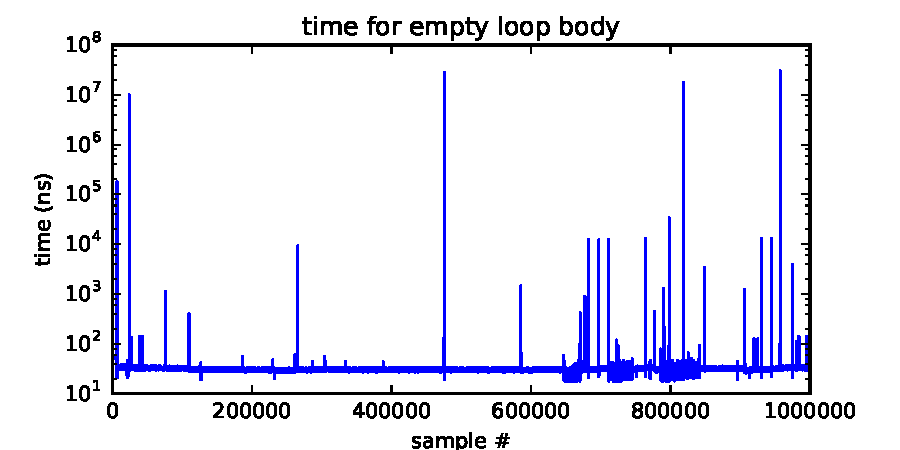
\includegraphics[width=\textwidth]{../kernel/empty-samples}
\end{frame}

\begin{frame}{doing nothing on a busy system}
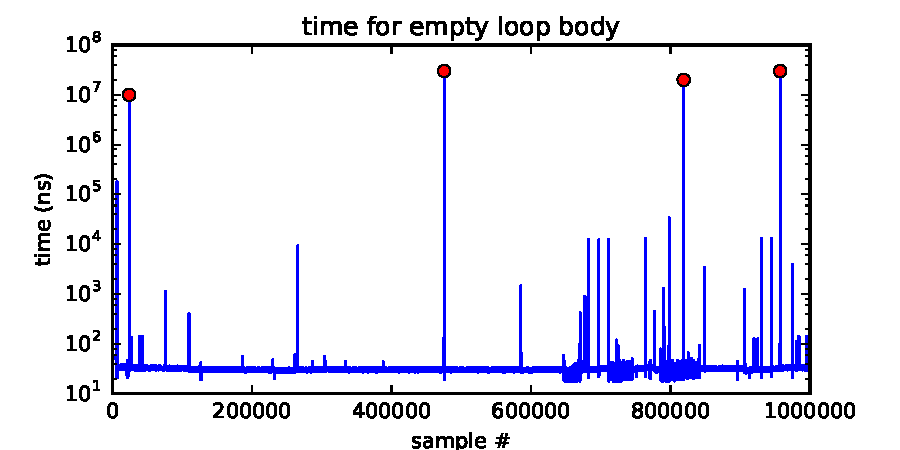
\includegraphics[width=\textwidth]{../kernel/empty-samples-big-marked}
\end{frame}



\section{time multiplexing}
\usetikzlibrary{arrows.meta}

\begin{frame}[fragile,label=timeMulti1]{time multiplexing}
\begin{tikzpicture}
\tikzset{
    prog1/.style={draw,fill=cyan!70},
    prog2/.style={draw,fill=green,visible on=<3->},
    prog3/.style={draw,fill=violet!30,visible on=<3->},
    proglabel/.style={font=\tt\scriptsize},
    labelprog1/.style={execute at begin node={\strut loop.exe}},
    labelprog2/.style={execute at begin node={\strut ssh.exe},visible on=<3->},
    labelprog3/.style={execute at begin node={\strut firefox.exe},visible on=<3->},
}

\begin{scope}[xscale=1.5,yscale=1]
\foreach \s/\e/\p [count=\x] in {0/2/1,2/3/2,3/5/3,5/6/1,6/7/2}{
    \draw[prog\p] (\s, 0) rectangle (\e, 1) coordinate[midway] (mid-\x);
    \node[anchor=center,proglabel,labelprog\p] at (mid-\x) {};
}
\end{scope}
\node[anchor=east] at (-0.25, 0.5) {CPU:};
% FIXME: system
\begin{scope}[yscale=1,yshift=-2.5mm]
\draw[thick,-Latex] (1,0) node[left] {time} -- (10.5,0);
\end{scope}
\begin{visibleenv}<2->
    \begin{scope}[xscale=1.5]
    \draw[red,thick] (1.9,-.1) coordinate (firstStart) rectangle (2.0, 1.1);
    \draw[red,thick] (5.1,-.1) coordinate (lastEnd) rectangle (5.0, 1.1);
    \end{scope}
    \node[anchor=north west] (asmPre) at (0, -1) {
\begin{lstlisting}[language=myasm,style=small]
...
call get_time 
    // whatever get_time does
movq %rax, %rbp
\end{lstlisting}
    };
    \draw[red, ultra thick] ([yshift=-.2cm]asmPre.south west) -- ([yshift=-.2cm]asmPre.south east) node [draw=none,midway,fill=white,
        inner sep=3pt] 
        {million cycle delay};
    \node[anchor=north west] (asmPost) at ([yshift=-.5cm]asmPre.south west) {
\begin{lstlisting}[language=myasm,style=small]
call get_time
    // whatever get_time does
subq %rbp, %rax
...
\end{lstlisting}
    };
\end{visibleenv}
\end{tikzpicture}
\end{frame}



\subsection{thread idea}
\begin{frame}{threads}
\begin{itemize}
\item thread = illusion of own processor
\vspace{.5cm}
\item own register values
\item own program counter value
\vspace{.5cm}
\item<2-> actual implementation: \\
    many threads sharing one processor
    \begin{itemize}
    \item problem: where are register/program counter values \\
        when thread not active on processor?
    \end{itemize}
\end{itemize}
\end{frame}



\section{reasons for exceptions, generally}
\usetikzlibrary{decorations.pathreplacing}

\begin{frame}<0>[label=exceptTypesN]{types of exceptions}
\begin{itemize}
\item \tikzmark{int bot}\myemph<3>{externally-triggered}
    \begin{itemize}
    \item \myemph<3>{timer} --- keep program from hogging CPU
    \item \myemph<4>{I/O devices} --- key presses, hard drives, networks, \ldots
    \item \tikzmark{abort bot}hardware is broken (e.g. memory parity error)
    \end{itemize}
\item \tikzmark{trap bot}intentionally triggered exceptions
    \begin{itemize}
    \item \myemph<5>{system calls} --- ask OS to do something
    \end{itemize}
\item \tikzmark{fault bot}\myemph<6>{errors/events in programs}
    \begin{itemize}
        \item \myemph<7>{memory not in address space} (``Segmentation fault'')
        \item \myemph<8>{privileged instruction}
    \item divide by zero
    \item invalid instruction\tikzmark{invalid}
    \end{itemize}
\end{itemize}
\begin{tikzpicture}[overlay,remember picture]
    \coordinate (int top) at ([yshift=.6cm]pic cs:int bot);
    \coordinate (fault top) at ([yshift=.6cm]pic cs:fault bot);
    \coordinate (trap top) at ([yshift=.6cm]pic cs:trap bot);
    \coordinate (fault bot) at (pic cs:fault bot);
    \coordinate (over) at ([xshift=-4.5cm]current page.east);
    \coordinate (abort bot)  at (pic cs:abort bot);
    \coordinate (invalid bot)  at ([yshift=.6cm]pic cs:invalid bot);
    \draw[very thick,decorate,decoration={brace}] (int top -| over) -- (abort bot -| over) 
        node[midway,right,font=\large] (async label) {\myemph<2>{asynchronous}};
        \node[anchor=north west,font=\small,align=left] at ([xshift=.15cm,yshift=.3cm]async label.south west) {
            not triggered by \\
            running program
        };
    \draw[very thick,decorate,decoration={brace}] (trap top -| over) -- (invalid bot -| over) 
        node[midway,right,font=\large] (sync label) {\myemph<2>{synchronous}};
        \node[anchor=north west,font=\small,align=left] at ([xshift=.15cm,yshift=.3cm]sync label.south west) {
            triggered by \\
            current program
        };
\end{tikzpicture}
\end{frame}

\againframe<1>{exceptTypesN}


\subsection{aside: terms}
\begin{frame}{terms for exceptions}
    \begin{itemize}
    \item terms for exceptions aren't standardized
    \vspace{.5cm}
    \item our readings use one set of terms
    \begin{itemize}
        \item interrupts = externally-triggered
        \item faults = error/event in program
        \item trap = intentionally triggered
        \end{itemize}
    \item all these terms appear differently elsewhere
    \end{itemize}
\end{frame}


\section{exception table + dispatch}

\begin{frame}{exception implementation}
\begin{itemize}
\item detect condition (program error or external event)
\item save current value of PC somewhere
\item jump to \myemph{exception handler} (part of OS)
    \begin{itemize}
    \item jump done without program instruction to do so
    \end{itemize}
\end{itemize}
\end{frame}

\begin{frame}{exception implementation: notes}
\begin{itemize}
\item I describe a \myemph{simplified} version
\item real x86/x86-64 is a bit more complicated
    \begin{itemize}
    \item (mostly for historical reasons)
    \end{itemize}
\end{itemize}
\end{frame}

\begin{frame}[label=locating,fragile]{locating exception handlers}
\begin{tikzpicture}
\tikzset{
    >=Latex,
    every node/.style={font=\small},
}
\matrix[tight matrix,
    nodes={text width=2.5cm,font=\small},
    column 1/.append style={nodes={draw=none}},
    column 2/.append style={nodes={text width=1.5cm}},
    row 1/.append style={nodes={draw=none}},
    label={[inner sep=0mm,align=center]north:{{\bfseries exception table} (in memory)}},
    label distance=1mm,
] (eTable) {
    |[align=center]| address \& pointer \\
    base + {\tt 0x00} \& ~ \\
    base + {\tt 0x08} \& ~ \\
    base + {\tt 0x10} \& ~ \\
    base + {\tt 0x18} \& ~ \\
    |[align=center]| \ldots \& |[draw=none,align=center]| \ldots \\
    base + {\tt 0x40} \&  ~ \\
    |[align=center]| \ldots \& |[draw=none,align=center]| \ldots \\
};
\node[draw,text width=2.8cm, align=center, anchor=south] (baseReg) at ([yshift=1cm,xshift=5mm]eTable-1-1.north west){ exception table base register };
\draw[dashed,very thick,->] ([xshift=-1.2cm]baseReg.south) |- (eTable-2-1.west);
\node[draw,anchor=north west] (hDivZero) at ([xshift=2cm,yshift=2cm]eTable-2-2.north east) {
\begin{lstlisting}[style=script,language=myasm]
handle_divide_by_zero:
  movq %rax, save_rax
  movq %rbx, save_rbx
  ...
\end{lstlisting}
};
\node[draw,anchor=north west] (hTimer) at ([yshift=-2.5cm]hDivZero.south west){
\begin{lstlisting}[style=script,language=myasm]
handle_timer_interrupt:
  movq %rax, save_rax
  movq %rbx, save_rbx
  ...
\end{lstlisting}
};
\draw[->,thick] (eTable-2-2.center) -- ++(2,0) |- ([yshift=-1ex]hDivZero.north west);
\draw[thick] (eTable-3-2.center) -- ++ (2, 0) node[right]{\ldots};
\draw[thick] (eTable-4-2.center) -- ++ (2, 0) node[right]{\ldots};
\draw[thick] (eTable-5-2.center) -- ++ (2, 0) node[right]{\ldots};
\draw[->,thick] (eTable-7-2.center) -- ++(2,0) |- ([yshift=-1ex]hTimer.north west);
\end{tikzpicture}
\end{frame}

\begin{frame}[fragile,label=exceptHandlerRun]{running the exception handler}
\begin{itemize}
    \item hardware saves the \myemph{old program counter} (and maybe more)
    \item identifies location of exception handler via table
    \item then jumps to that location
    \vspace{.5cm}
    \item OS code can save anything else it wants to , etc.
\end{itemize}
\end{frame}




\section{context switches} % FIXME: move earlier???
    % FIXME: simplify diagram
    % FIXME: include address space as part of context
\usetikzlibrary{arrows.meta,calc,positioning,matrix,patterns}

\begin{frame}{switching programs}
% FIXME: picture showing zoom of timeline
\begin{itemize}
\item OS starts running somehow
    \begin{itemize}
    \item some sort of exception
    \end{itemize}
\item saves old registers + program counter + address mapping
    \begin{itemize}
    \item (optimization: could omit when program crashing/exiting)
    \end{itemize}
\item sets new registers + address mapping, jumps to new program counter
\item called \myemph{context switch}
    \begin{itemize}
    \item saved information called \myemph{context}
    \end{itemize}
\end{itemize}
\end{frame}

\tikzset{a/.style={fill=blue!10,pattern=north west lines,pattern color=blue!30},b/.style={fill=green!30},>=Latex}
\newsavebox{\aContext}
\savebox{\aContext}{
\begin{tikzpicture}
\matrix[tight matrix,nodes={font=\small\tt,a}] (cpuState) {
    \%rax \& SF \\
    \%rbx \& ZF \\
    \%rcx \& PC \\
    \ldots \& \ldots \\
};
\end{tikzpicture}
}
\newsavebox{\bContext}
\savebox{\bContext}{
\begin{tikzpicture}
\matrix[tight matrix,nodes={font=\small\tt,b}] (cpuState) {
    \%rax \& SF \\
    \%rbx \& ZF \\
    \%rcx \& PC \\
    \ldots \& \ldots \\
};
\end{tikzpicture}
}


\begin{frame}{contexts (A running)}
\begin{tikzpicture}
\matrix[tight matrix,label={north:in CPU},nodes={font=\small\tt,a}] (cpuState) {
    \%rax \\
    \%rbx \\
    \%rcx \\
    \%rsp \\
    \ldots \\
    SF \\
    ZF \\
    PC \\
};

\matrix[tight matrix,right=3cm of cpuState, nodes={minimum height=2cm,text width=5cm,align=left},label={in Memory}] (memState) {
    |[a]| {Process A memory: \\ code, stack, etc.} \\
    |[b]| {Process B memory: \\ code, stack, etc.} \\
    |[fill=black!10]|{OS memory: \\ \usebox{\bContext} }\\
};
\draw[thick,dashed,->] (cpuState-4-1.east) -- (memState-1-1.west);
\draw[thick,dashed,->] (cpuState-8-1.east) -- (memState-1-1.west);
\end{tikzpicture}
\end{frame}

\begin{frame}{contexts (B running)}
\begin{tikzpicture}
\tikzset{a/.style={fill=blue!10,pattern=north west lines,pattern color=blue!30},b/.style={fill=green!30},>=Latex}
\matrix[tight matrix,label={north:in CPU},nodes={font=\small\tt,b}] (cpuState) {
    \%rax \\
    \%rbx \\
    \%rcx \\
    \%rsp \\
    \ldots \\
    SF \\
    ZF \\
    PC \\
};
\matrix[tight matrix,right=3cm of cpuState, nodes={minimum height=2cm,text width=5cm},label={north:in Memory}]
    (memState) {
    |[a]| {Process A memory: \\ code, stack, etc.} \\
    |[b]| {Process B memory: \\ code, stack, etc.} \\
    |[fill=black!10]| {OS memory: \\ \usebox{\aContext}} \\
};
\draw[thick,dashed,->] (cpuState-4-1.east) -- (memState-2-1.west);
\draw[thick,dashed,->] (cpuState-8-1.east) -- (memState-2-1.west);
\end{tikzpicture}
\end{frame}




\section{exercise}
\begin{frame}{which of these require exceptions? context switches?}
    \begin{itemize}
    \item A. program calls a function in the standard library
    \item B. program writes a file to disk
    \item C. program A goes to sleep, letting program B run
    \item D. program exits
    \item E. program returns from one function to another function
    \item F. program pops a value from the stack
    \end{itemize}
\end{frame}

\iftoggle{heldback}{}{
\begin{frame}{which require exceptions [answers] (1)}
\begin{itemize}
    \item A. program calls a function in the standard library
        \begin{itemize}
        \item no (same as other functions in program; some standard library functions might make system calls, but if so, that'll be part of what happens after they're called and before they return)
        \end{itemize}
    \item B. program writes a file to disk
        \begin{itemize}
        \item yes (requires kernel mode only operations)
        \end{itemize}
    \item C. program A goes to sleep, letting program B run
        \begin{itemize}
        \item yes (kernel mode usually required to change the address space to acess program B's memory)
        \end{itemize}
\end{itemize}
\end{frame}
\begin{frame}{which require exceptions [answer] (2)}
    \begin{itemize}
    \item D. program exits
        \begin{itemize}
        \item yes (requires switching to another program, which requires accessing OS data + other program's memory)
        \end{itemize}
    \item E. program returns from one function to another function
        \begin{itemize}
        \item no
        \end{itemize}
    \item F. program pops a value from the stack
        \begin{itemize}
        \item no
        \end{itemize}
    \end{itemize}
\end{frame}

\begin{frame}{which require context switches [answer]}
    \begin{itemize}
    \item no: A. program calls a function in the standard library
    \item no: B. program writes a file to disk
        \begin{itemize}
        \item (but might be done if program needs to wait for disk and other things could be run while it does)
        \end{itemize}
    \item yes: C. program A goes to sleep, letting program B run
    \item yes: D. program exits
    \item no: E. program returns from one function to another function
    \item no: F. program pops a value from the stack
    \end{itemize}
\end{frame}
}


\section{process}
\begin{frame}{The Process}
\begin{itemize}
\item \myemph{process} = thread(s) + address space
\item illusion of \myemph{dedicated machine}:
\begin{itemize}
\item thread = illusion of own CPU
\item address space = illusion of own memory
\end{itemize}
\end{itemize}
\end{frame}


\end{document}


\section{backup slides}
\begin{frame}{backup slides}
\end{frame}

\subsection{suffix rules}

\begin{frame}{suffix rules}

{\tt
\begin{tabular}{l}
CC = gcc \\
CFLAGS = -Wall \\
LDFLAGS = -Wall \\
~ \\
program: main.o extra.o \\
▶\hspace{1.5cm}\$(CC) \$(LDFLAGS) -o {\$@} {\$\textasciicircum} \\
~ \\
\myemph{.c.o:} \\
▶\hspace{1.5cm}\$(CC) \$(CFLAGS) -o {\$@} -c {\$<} \\
~ \\
extra.o: extra.c extra.h \\
main.o: main.c main.h extra.h \\
\myemph{.SUFFIXES: .c .o} \\
\end{tabular}
} \\
{\small aside: \texttt{\$\textasciicircum} works on GNU make (usual on Linux), but not portable.}
\end{frame}




\subsection{exercise with custom compiler}
\begin{FragileFrame}
\frametitle{exericse setup}
    \begin{itemize}
    \item a program has source files compiler.c, main.c, functions.customlang
    \item compiler.c builds a custom compiler
    \item functions.customlang needs to be compiled with that compiler
    \item so normal build process is:
\begin{Verbatim}[frame=single,fontsize=\fontsize{12}{13}]
clang -c compiler.c
clang -c main.c
clang -o compiler compiler.o
./compiler -c functions.customlang
clang -o program main.o functions.o
\end{Verbatim}
    \end{itemize}
\end{FragileFrame}

\begin{FragileFrame}
\frametitle{exercise part 1}
\begin{Verbatim}[frame=single,fontsize=\fontsize{13}{14}]
clang -c compiler.c
clang -c main.c
clang -o compiler compiler.o
./compiler -c functions.customlang
clang -o program main.o functions.o
\end{Verbatim}
    \begin{itemize}
    \item besides \texttt{program}, \texttt{main.o}, makefile should have what targets?
\begin{tabular}{ll}
    A. \texttt{functions.customlang} & B. \texttt{functions.o} \\
    C. \texttt{compiler.o} & D. \texttt{compiler} \\
    E. all of the above & F. B and C \\
    G. A and B and D & H. B and C and D \\
    I. something else 
\end{tabular}
    \end{itemize}
\end{FragileFrame}

\begin{FragileFrame}
\frametitle{exercise part 2}
\begin{Verbatim}[frame=single,fontsize=\fontsize{12}{13}]
clang -c compiler.c
clang -c main.c
clang -o compiler compiler.o
./compiler -c functions.customlang
clang -o program main.o functions.o
\end{Verbatim}
    \begin{itemize}
    \item part 2: make rule for functions.o? first blank = ???
\begin{Verbatim}[frame=single,fontsize=\fontsize{11}{12}]
functions.o: ____________________________________
▶     _____________________________________
\end{Verbatim}
\begin{tabular}{llll}
A. & \texttt{functions.customlang} & B. & \texttt{functions.customlang compiler} \\
C. & \texttt{compiler} & D. & \texttt{functions.customlang compiler.o} \\
E. & \texttt{functions.c} & F. & \texttt{program} \\
G. & something else\\
\end{tabular}
    \end{itemize}
\end{FragileFrame}

\begin{FragileFrame}
\frametitle{exercise part 3}
\begin{Verbatim}[frame=single,fontsize=\fontsize{13}{14}]
clang -c compiler.c #1
clang -c main.c #2
clang -o compiler compiler.o #3
./compiler -c functions.customlang #4
clang -o program main.o functions.o #5
\end{Verbatim}
    \begin{itemize}
    \item command 1 goes in rule for which target? command 3? 4?
\begin{tabular}{lll}
    A. \texttt{compiler.o} & B. \texttt{main.o} & C. \texttt{compiler} \\
    D. \texttt{functions.o} & E. \texttt{program} & F. something else \\
\end{tabular}
    \end{itemize}
\end{FragileFrame}




\section{permissions exercise}
\begin{frame}{exercise}
\begin{itemize}
\item \texttt{foo/bar/baz} (all directories)
    \begin{itemize}
    \item \texttt{foo}: owner 613; group 75; permissions \texttt{0755}
    \item \texttt{bar}: owner 1219; group 75; permissions \texttt{0750}
    \item \texttt{baz}: owner 1219; group 75; permissions \texttt{0730}
    \end{itemize}
\item users 613+1219s processes are part of group 75
\item (1 = execute/search; 2 = write; 4 = read)
\item which will work?
    \begin{itemize}
    \item user 613 does \texttt{ls -l foo}
    \item user 613 does \texttt{ls foo/bar}
    \item user 613 writes \texttt{foo/bar/quux}
    \item user 613 deletes \texttt{foo/bar/baz}
    \end{itemize}
\end{itemize}
\end{frame}


\section{authentication v authorization}
\begin{frame}{authorization v authentication}
    \begin{itemize}
    \item \textit{authentication} --- who is who
    \vspace{.5cm}
    \item<2-> \textit{authorization} --- who can do what
        \begin{itemize}
        \item probably need authentication first\ldots
        \end{itemize}
    \end{itemize}
\end{frame}

\begin{frame}{authentication}
    \begin{itemize}
    \item password
    \item hardware token
    \item \ldots
    \vspace{.5cm}
    \item<2-> this class: mostly won't deal with how
    \item<2-> just tracking afterwards
    \end{itemize}
\end{frame}



\section{exercises on the POSIX model}
\begin{frame}[label=secTasks1]{some security tasks (1)}
    \begin{itemize}
    \item helping students collaborate in ad-hoc small groups on shared server?
    \vspace{.5cm}
    \item Q1: what to allow/prevent?
    \item Q2: how to use POSIX mechanisms to do this?
    \end{itemize}
\end{frame}

\begin{frame}[label=secTasks2]{some security tasks (2)}
    \begin{itemize}
    \item letting students assignment files to faculty on shared server?
    \vspace{.5cm}
    \item Q1: what to allow/prevent?
    \item Q2: how to use POSIX mechanisms to do this?
    \end{itemize}
\end{frame}

\begin{frame}[label=secTasks3]{some security tasks (3)}
    \begin{itemize}
    \item running untrusted game program  from Internet?
    \vspace{.5cm}
    \item Q1: what to allow/prevent?
    \item Q2: how to use POSIX mechanisms to do this?
    \end{itemize}
\end{frame}


\subsection{setuid ``gates''}

\begin{frame}{set-user ID gates}
\begin{itemize}
\item set-user ID program: gate to higher privilege
\vspace{.5cm}
\item controlled access to extra functionality
\item make authorization/authentication decisions \textit{outside the kernel}
\item way to allow normal users to do \textit{one thing that needs privileges}
    \begin{itemize}
    \item write program that does that one thing --- nothing else!
    \item make it owned by user that can do it (e.g. root)
    \item mark it set-user-ID
    \end{itemize}
\item want to allow only some user to do the thing
    \begin{itemize}
    \item make program check which user ran it
    \end{itemize}
\end{itemize}
\end{frame}


\begin{frame}{set-user-ID program v syscalls}
\begin{itemize}
\item hardware decision: some things only for kernel
\item system calls: \textit{controlled} access to things kernel can do
\item decision about how can do it: in the kernel
\vspace{.5cm}
\item kernel decision: some things only for root (or other user)
\item set-user-ID programs: controlled access to things root/\ldots{} can do
\item decision about how can do it: made by root/\ldots
\end{itemize}
\end{frame}



\subsection{buggy set-user-ID program 1}
\begin{frame}{a broken setuid program: setup}
    \begin{itemize}
    \item suppose I have a directory all-grades on shared server
    \item in it I have a folder for each assignment
    \item and within that a text file for each user's grade + other info
    \item say I don't have flexible ACLs and want to give each user access
    \vspace{.5cm}
    \item<2-> one (bad?) idea: setuid program to read grade for assignment
    \item<2-> \texttt{./print\_grade assignment}
    \item<2-> outputs grade from \texttt{all-grades/assignment/USER.txt}
    \end{itemize}
\end{frame}

\begin{frame}[fragile,label=brokenSetuid]{a very broken setuid program}
print\_grade.c:
\begin{lstlisting}[language=C,style=small]
int main(int argc, char **argv) {
    char filename[500];
    sprintf(filename, "all-grades/%s/%s.txt",
            argv[1], getenv("USER"));
    int fd = open(filename, O_RDWR);
    char buffer[1024];
    read(fd, buffer, 1024);
    printf("%s: %s\n", argv[1], buffer);
}
\end{lstlisting}
\begin{itemize}
\item HUGE amount of stuff can go wrong
\item examples?
\end{itemize}
\end{frame}


\subsection{other privilege escalation contexts}
\begin{frame}{other privileged escalation issues}
    \begin{itemize}
    \item sudo problem: trusted code that's supposed to enforce restriction \\
        can be fooled into not really enforcing it
    \item also can occur in other contexts:
    \vspace{.5cm}
    \item system call letting program access things it shouldn't?
    \item browser letting web page javascript access things it shouldn't?
    \item web application giving users access to files they shouldn't have?
    \item mobile phone OS allowing location access without location permission?
    \item \ldots
    \end{itemize}
\end{frame}


\subsection{buggy set-user-ID program 2}
\begin{frame}{another very broken setuid program (setup)}
\begin{itemize}
\item allow users to print files, but only if less than 1KB
\end{itemize}
\end{frame}


\begin{frame}[fragile]{another very broken setuid program}
\lstset{language=C,style=small}
print\_short\_file.c:\\
\begin{lstlisting}[language=C,style=small]
int main(int argc, char **argv) {
    struct stat st;
    if (stat(argv[1], &st) == -1) abort();
    // make sure argv[1] is owned by user running this
    if (st.st_uid != getuid()) abort();
    // and that it's less than 1 KB
    if (st.st_size >= 1024) abort();
    char command[1024];
    sprintf(command, "print %1000s", argv[1]);
    system(command);
    return EXIT_SUCCESS;
}
\end{lstlisting}
\end{frame}



\subsection{TOCTTOU example}

\begin{frame}{a delegation problem}
\begin{itemize}
\item consider printing program marked setuid to access printer
    \begin{itemize}
    \item decision: no accessing printer directly
    \item printing program enforces page limits, etc.
    \end{itemize}
\item command line: file to print
\item can printing program just call open()?
\end{itemize}
\end{frame}

\begin{frame}[fragile,label=delegationBroken]{a broken solution}
\begin{lstlisting}[language=C++,style=small]
if (original user can read file from argument) {
    open(file from argument);
    read contents of file;
    write contents of file to printer
    close(file from argument);
}
\end{lstlisting}
\begin{itemize}
\item hope: this prevents users from printing files than can't read
\item problem: race condition!
\end{itemize}
\end{frame}

\begin{frame}[fragile,label=delegationBrokenWhy]{a broken solution / why}
\begin{tabular}{l|l}
setuid program & other user program \\ \hline
                & create normal file \texttt{toprint.txt} \\
check: can user access? (yes)  & --- \\
~ & \texttt{unlink("toprint.txt")} \\
~ & \texttt{link("/secret", "toprint.txt")} \\
\texttt{open("toprint.txt")} & --- \\
read \ldots & --- \\
\end{tabular}
\begin{itemize}
\item link: create new directory entry for file
    \begin{itemize}
    \item another option: rename, symlink (``symbolic link'' --- alias for file/directory)
    \item another possibility: run a program that creates secret file \\
        (e.g. temporary file used by password-changing program)
    \end{itemize}
\item time-to-check-to-time-of-use vulnerability
\end{itemize}
\end{frame}

\begin{frame}{TOCTTOU solution}
\begin{itemize}
\item temporarily `become' original user
\item then open
\item then turn back into set-uid user
\vspace{.5cm}
\item this is why POSIX processes have multiple user IDs
\item can swap out effective user ID temporarily
\end{itemize}
\end{frame}

\begin{frame}{practical TOCTTOU races?}
    \begin{itemize}
    \item can use symlinks \textit{maze} to make check slower
    \begin{itemize}
        \item symlink \texttt{toprint.txt} $\rightarrow$ \texttt{a/b/c/d/e/f/g/normal.txt}
        \item symlink \texttt{a/b} $\rightarrow$ \texttt{../a}
        \item symlink \texttt{a/c} $\rightarrow$ \texttt{../a}
        \item \ldots
    \end{itemize}
    \item lots of time spent following symbolic links when program opening toprint.txt
    \item gives more time to sneak in unlink/link or (more likely) rename
    \end{itemize}
\end{frame}


\subsubsection{exercise}

\begin{frame}{exercise}
    \begin{itemize}
    \item which (if any) of the following would fix for a TOCTTOU vulnerability in our setuid printing application?
        (assume the Unix-permissions without ACLs are in use)
    \vspace{.5cm}
    \item\relax[A] \textbf{both before and after} opening the path passed in for reading, check that the path is accessible to the user who ran our application
    \item\relax[B] after opening the path passed in for reading, using \texttt{fstat} with the file descriptor opened to check the permissions on the file
    \item\relax[C] before opening the path, verify that the user controls the file referred to by the path \textbf{and} the directory containing it
    \end{itemize}
\end{frame}
 % FIXME: add to zoom


\section{backup slides}
\begin{frame}{backup slides}
\end{frame}

\end{document}
